\startcontents[localtoc]
\printcontents[localtoc]{}{0}{\subsection*{Contents}\setcounter{tocdepth}{2}}



\phantomsection
\addcontentsline{toc}{section}{Generate sample data}
\subsubsection*{Generate sample data}



Two quantities are prepared: \texttt{x} and \texttt{y}.

\begin{lstlisting}
x = []; y = [];
x.v = [1:20];
y.v = [1:14 13:-1:8];
\end{lstlisting}


All uncertainties are set to 1.

\begin{lstlisting}
x.u = x.v.*0 + 1;
y.u = y.v.*0 + 1;
\end{lstlisting}


Set degrees of freedom.

\begin{lstlisting}
x.d = x.v.*0 + 60;
y.d = y.v.*0 + 9;
\end{lstlisting}


Quantities are put into data input structure \texttt{DI}.

\begin{lstlisting}
DI = [];
DI.x = x;
DI.y = y;
\end{lstlisting}


Create calculation settings \texttt{CS} and set uncertainty calculation method to Monte Carlo method.
Allow randomization of uncertainties by the QWTB toolbox.

\begin{lstlisting}
CSMCM = [];
CSMCM.unc = 'mcm';
CSMCM.mcm.randomize = 1;
\end{lstlisting}


Create calculation settings and set uncertainty calculation method to GUM uncertainty framework.

\begin{lstlisting}
CSGUF = [];
CSGUF.unc = 'guf';
\end{lstlisting}


\phantomsection
\addcontentsline{toc}{section}{Call algorithm}
\subsubsection*{Call algorithm}



Use QWTB to apply algorithm \texttt{testGM} to data \texttt{DI} with calculation settings \texttt{CSGUF}.

\begin{lstlisting}
DOGUF = qwtb('testGM', DI, CSGUF);
\end{lstlisting}
\begin{lstlisting}[language={},xleftmargin=5pt,frame=none]
QWTB: default correlation matrix generated for quantity `x`
QWTB: default correlation matrix generated for quantity `y`
QWTB: uncertainty calculation by means of wrapper or algorithm

\end{lstlisting}


Use QWTB to apply algorithm \texttt{testGM} to data \texttt{DI} with calculation settings \texttt{CSMCM}.

\begin{lstlisting}
DOMCM = qwtb('testGM', DI, CSMCM);
\end{lstlisting}
\begin{lstlisting}[language={},xleftmargin=5pt,frame=none]
QWTB: default correlation matrix generated for quantity `x`
QWTB: default correlation matrix generated for quantity `y`
QWTB: uncertainty calculation by means of wrapper or algorithm

\end{lstlisting}


\phantomsection
\addcontentsline{toc}{section}{Plot results}
\subsubsection*{Plot results}



Plot input data and calculated maximal and minimal values as a red and green lines with
uncertainties represented by dashed lines.

\begin{lstlisting}
figure
hold on
errorbar(DI.x.v, DI.y.v, DI.y.u, 'xb')
plot([DI.x.v(1) DI.x.v(end)], [DOGUF.max.v DOGUF.max.v], '-r', 'linewidth', 3)
plot([DI.x.v(1) DI.x.v(end)], [DOGUF.max.v - DOGUF.max.u DOGUF.max.v - DOGUF.max.u], '--r', 'linewidth', 3)
plot([DI.x.v(1) DI.x.v(end)], [DOGUF.min.v DOGUF.min.v], '-g', 'linewidth', 3)
plot([DI.x.v(1) DI.x.v(end)], [DOGUF.min.v - DOGUF.min.u DOGUF.min.v - DOGUF.min.u], '--g', 'linewidth', 3)
plot([DI.x.v(1) DI.x.v(end)], [DOGUF.max.v + DOGUF.max.u DOGUF.max.v + DOGUF.max.u], '--r', 'linewidth', 3)
plot([DI.x.v(1) DI.x.v(end)], [DOGUF.min.v + DOGUF.min.u DOGUF.min.v + DOGUF.min.u], '--g', 'linewidth', 3)
legend('original data (DI.x.v, DI.y.v)', 'line at maximum value (DO.max.v)', 'uncertainty',  'line at minimum value (DO.min.v)', 'uncertainty', 'location', 'southoutside')
xlabel('quantity x')
ylabel('quantity y')
title('input data and results of testGM algorithm, GUF method')
hold off
\end{lstlisting}
\begin{center}
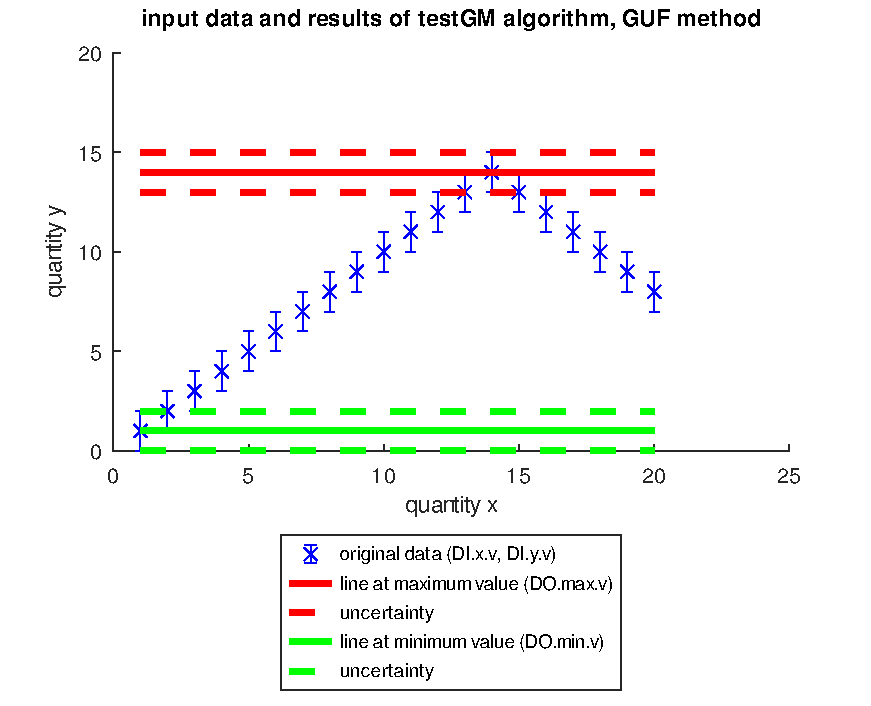
\includegraphics[width=0.7\textwidth]{algs_examples_published/testGM_alg_example-1.pdf}
\end{center}


Plot histogram of calculated maximal value, i.e. probability density function simulated by Monte
Carlo method and overlay by result of GUF method (approximately scaled to MCM result).

\begin{lstlisting}
figure
hold on
hist(DOMCM.max.r, 50)
a = axis;
x = [a(1):0.1:a(2)];
pdf = normpdf(x, DOGUF.max.v, DOGUF.max.u);
plot(x, a(4)/max(pdf).*pdf, '-r', 'linewidth', 4);
title('results of maximum value (DO.max.r)')
legend('Monte Carlo results', 'GUF result (approximately scaled to MCM results', 'location', 'southoutside')
hold off
\end{lstlisting}
\begin{center}
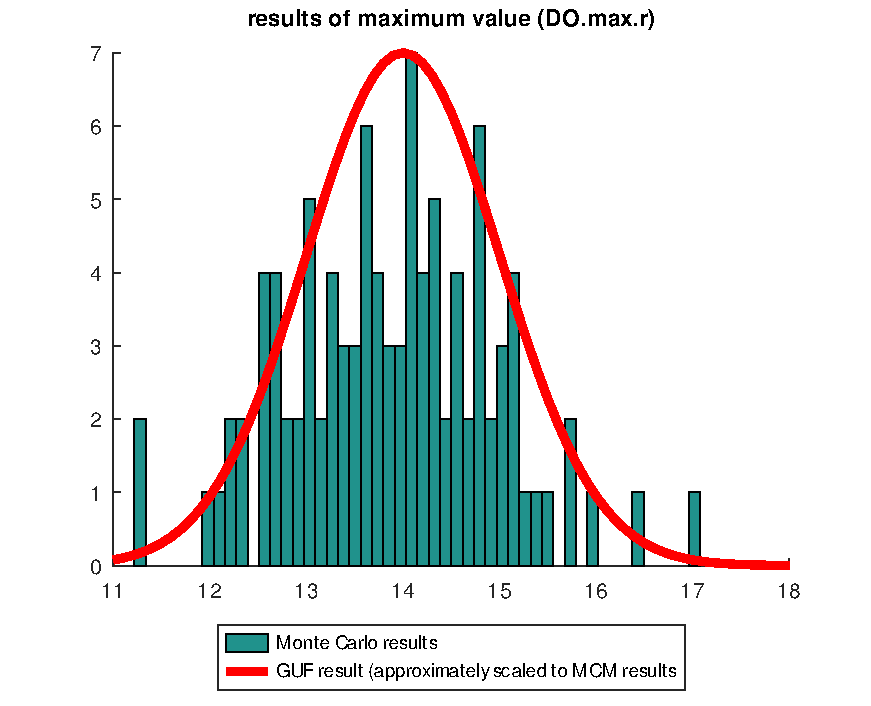
\includegraphics[width=0.7\textwidth]{algs_examples_published/testGM_alg_example-2.pdf}
\end{center}


\stopcontents[localtoc]
